\begin{definition}[Subgrupo característico]
  Seja $G$ um grupo e $\varphi:G\to G$ com $\varphi\in Aut(G)$. Se $H\leq G$ implica que $\varphi(H)\leq H$ para todo $\varphi\in Aut(G)$ dizemos que $H$ é um subgrupo \textbf{característico} de $G$ e denotamos por $H\car G$. 
\end{definition}
\begin{note}
  Se $H\car G$, então em particular $\phi_g(H)\leq H$, logo $gH=Hg$ para todo $g\in G$, i.e, $H\normal G$.\\
  Mas na reciproca não é necesariamente verdadeira.
\end{note}
\begin{example}
  Seja $G=K_4=\{1,a,b,ab\}=\left\langle a,b:a^{2}=1,b^{2}=1,ab=ba \right\rangle$, lembre que
  \begin{center}
    \input{images/k4subgrupos}
  \end{center}
  logo $\left\langle a \right\rangle\normal K_4$, mas $b\left\langle a \right\rangle\cnot\leq H$, logo $\left\langle a \right\rangle \cnot\car K_4$.
\end{example}
Note que a normalidade não é transitiva, suponha $H,K\leq G$ , com $H\normal K$ e $K\normal G$, logo não necesariamente $H\normal G$.
\begin{example}
  Seja $G=D_4=\left\langle r,\theta:r^{2}=\theta^{4}=1,r\theta=\theta^{-1}r \right\rangle$, logo $\left\langle r \right\rangle\normal \left\langle r,\theta^{2} \right\rangle$ e $\left\langle r,\theta^{2} \right\rangle\normal D_4$, mas $\left\langle r \right\rangle\cnot\normal D_4$.\\
  \textcolor{red}{Fazer diagrama}.
\end{example}
\begin{proposition}[Propriedades do subgrupos característicos]
  Seja $H,K\leq G$, então
  \begin{enumerate}
    \item $H\car K$, $K\car G$, então $H\car G$.
    \item $H\car K$, $K\normal G$, então $H\normal G$.
    \item $H\normal K$, $K\car G$, então $H\normal G$.
  \end{enumerate}
\end{proposition}
\begin{example}
  Note que para todo $\varphi\in Aut(G)$ temos que $\varphi(Z(G))\leq Z(G)$.
\end{example}
\begin{definition}[Grupo maximal]
  Um subgrupo $M\leq G$ é dito \textbf{maximal} se $M\neq G$ e se $H\leq G$ é tal que $M\leq H\leq G$, então $H=M$ ou $H=G$. 
\end{definition}
\begin{definition}[Grupo de Frattini]
  Seja $G$ um grupo, denotamos por $\phi(G)$ al \textbf{grupo de Frattini} de $G$ definido por
  \begin{align*}
    \phi(G)=\bigcap_{M\leq G},\quad\text{onde $M$ é maximal.}
  \end{align*}
\end{definition}
\begin{example}
  Seja $G$ grupo, então $\phi(G)\car G$. 
\end{example}
\begin{definition}[Conmutado]
  Dado $x,y\in G$, denotamos $[x,y]$ al \textbf{conmutador de $x$ e $y$} definido por 
  \begin{align*}
    [x,y]=x^{-1}y{-1}xy.
  \end{align*}
  Note que $[x,y]=1$ se, somente se, $x$ e $y$ conmutan. 
\end{definition}
\begin{definition}[Grupo derivado]
  Se $G$ é um grupo, denotamos $G^{\prime}$ al \textbf{grupo derivado de $G$} definido por
  \begin{align*}
    G^{\prime}=\left\langle [x,y]:x,y\in G \right\rangle.
  \end{align*}
\end{definition}
\begin{example}
  Note que $[x,y]^{-1}=[y,x]$ e $G^{\prime}\car G$.\\
  Basta mostrar que dada $\varphi\in Aut(G)$, então $\varphi([x,y])\in G$ para todo $x,y\in G$ e $\varphi([x,y])=[\varphi(x),\varphi(y)]$.\\
  Então, temos que $G^{\prime}\normal G$ e também temos que $G/G^{\prime}$ é um grupo abeliano.\\
  Alem disso, se $N\normal G$ é tal que $G/N$ é abeliano, então $G^{\prime}\leq N$. 
\end{example}
\begin{example}
  Seja $G=S_3$, logo $Z(S_3)=\{1\}$, vamos calcular $S_3^{\prime}$, lembremos o diagrama do note \ref{note:subgrupos-s3} 
  \begin{center}
    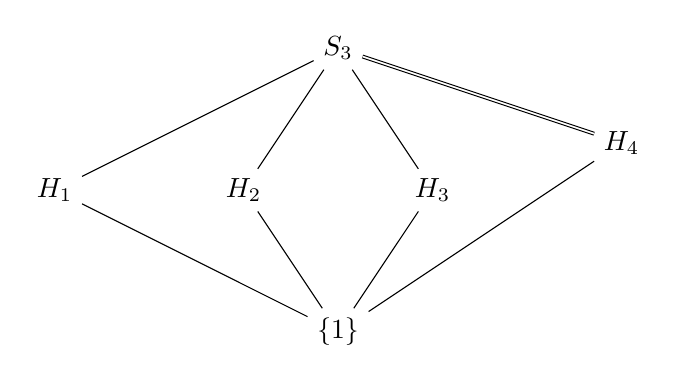
\begin{tikzpicture}[scale=1.2]
  % Nodes
  \node (S3) at (0,3) {$S_3$};

  \node (H1) at (-3,1.5) {$H_1$};
  \node (H2) at (-1,1.5) {$H_2$};
  \node (H3) at (1,1.5) {$H_3$};
  \node (H4) at (3,2) {$H_4$};

  \node (e) at (0,0) {$\{1\}$};

  % Edges from top
  \draw (S3) -- (H1);
  \draw (S3) -- (H2);
  \draw (S3) -- (H3);

  % Double line for normal subgroup
  \draw[double] (S3) -- (H4);

  % Edges to trivial subgroup
  \draw (H1) -- (e);
  \draw (H2) -- (e);
  \draw (H3) -- (e);

  % Double line again for normal chain
  \draw (H4) -- (e);
\end{tikzpicture}
  
  \end{center}
  Note que $S_3^{\prime}\normal S_3$, logo $S^{\prime}=H_4$ ou $S_3^{\prime}=S_3$, mas $|S_3/H_4|=2$, então $S_3/H_4$ é abeliano, portanto $S_3^{\prime}\leq H_4$, i.e, $S_3^{\prime}=H_4$. 
\end{example}
